\section{Technical preliminaries}
\label{preliminaries}
Let $S$ be a set. 
A \emph{trace} is an infinite sequence $\delta\in S^\omega$.
For a model $M$ with state space $S$, the reachable behavior space of the model $M$ is denoted as $\beh(M)\subset S^\omega$. 
Let $Var(M)$ be the set of variables of model $M$.
Then $AP$ is a set of \emph{atomic propositions} $p$, which are expressions on $Var(M)$, e.g. $p \defeq V_1 + V_2 > 4$ where $V_i \in Var(M)$.
Let $Var(p)$ be the set of variables that appear in the atomic proposition $p$.
Given a formula $\varphi$ on $AP$ in some logic, $Var(\varphi) = \cup_{p \textrm{ in }\varphi} Var(p)$.

A formula $\varphi$ defines a region in $\beh(M)$ within which the formula is satisfied, which can be denoted as $\beh(\varphi)$.
A \emph{model checker} takes a system model $M$ and a formal requirement $\varphi$, and returns whether $\beh(M) \subset \beh(\varphi)$, which is denoted by $M\models\varphi$. 
If the inclusion doesn't hold, the model checker returns a \emph{counter-example} $\delta_v\in\beh(M) \setminus \beh(\varphi)$.
This counter-example is used by the designer to debug the problem. 

%\subsection{Model Abstraction with Over-approximation}
%\label{overapx}
%\hatodo{save spce by not making this a separate subsection.}
%%The behavior space of the actual system is too large for model checker to exhaustively explore. 
%A model of the system that covers all behaviors of the system can be developed which can not only reduce complexity, but also having the suitable formalism for the model checker. 
%\hatodo{Previous statement is too vague: "suitable"? Might be best to remove it.}
An abstraction function $\absfun$ abstracting model $M$ to $M'$ is a function from state space $S$ to the new abstract state space $S'$ such that: 
%\hatodoin{removed non-surjective because it's not necessary for over-approximation. See Fig.1 in Clarke's JACM paper: his function is surjective, but still introduces over-approximation.}
$$\forall s\in S, \exists s'\in S' \text{ s.t. } \absfun(s)=s'$$
This definition can be extended to behaviors $\delta\in \mathbb{B}(M)$, such that:
$$\forall \delta\in \mathbb{B}(M),\exists \delta'\in\mathbb{B}(M')\text{ s.t. } \absfun(\delta)=\delta'$$
From the definition, we know that the more abstract model $M'$ covers all behaviors of $M$, which is referred to as \emph{over-approximation}. 
The over-approximation relationship is denoted as $M\triangleleft_h M'$, and the relationship between reachable behavior spaces as $\absfun(\mathbb{B}(M))\subseteq\mathbb{B}(M')$. 

Let $\varphi$ be a requirement on $M$ expressed in ATCTL$^*$, and $\absfun$ be an abstraction function. The model $\absfun(M)$ is \emph{appropriate} for the requirement $\varphi$ if 
	$\absfun(M) \models \varphi \implies M \models \varphi$. 
	

%With a requirement $\varphi$ in $ATCTL^*$\hatodo{what's this logic? give a reference}, we have:
%$$\absfun(\mathbb{B}(M))\subseteq \mathbb{B}(M'),\mathbb{B}(M')\subseteq \mathbb{B}(\varphi) \Rightarrow \absfun(\mathbb{B}(M))\subseteq \mathbb{B}(\varphi)\Rightarrow M\models\varphi$$
%\hatodoin{the last implication requires appropriateness, it doesn't follow automatically for any abstraction function}
%In general the state space of $S'$ is smaller than $S$ while preserving the property, thus preferable during model checking. 
%\hatodoin{I'm concerned that stressing that over-apx reduces the state space is the wrong emphasis: we don't use abstraction to reduce the tate space because our models are very small. We use to cover new behaviors.}
%\hatodoin{Also, be vareful: your state spaces are infinite, so what does it mean that one is smaller than the other? I suggest not making incomplete arguments here, just define things.}

Over-approximation can also be used to cover the behaviors of multiple models. 
A model $M'$ is an over-approximation of model $M_1$ and $M_2$ if 
$$\forall \delta\in \mathbb{B}(M_1)\cup\mathbb{B}(M_2),\exists \delta'\in\mathbb{B}(M')\text{ s.t. } \absfun(\delta)=\delta'$$
which is denoted as $\{M_1,M_2\}\triangleleft_h M'$, such that $\absfun(\mathbb{B}(M_1)\cup\mathbb{B}(M_2))\subseteq\mathbb{B}(M')$.


%\subsection{Appropriateness of a Model for a Requirement}
The state of a model $M$ is represented as $s=(s_1,s_2\cdots s_n)$ in which $s_i, i\in [1,n]$ are the substates. We use $Var(M)={s_1,s_2\cdots s_n}$ to represent all the substates variables in $M$. For an abstraction function $h$ which removes $s_i$ from the substates, we have:
$$\forall s_j,j\in [1,n], h(s_1,s_2\cdots s_n)=(s_1\cdots s_{i-1},s_{i+1}\cdots s_n)$$
It shows that $h$ is an over-approximation and in the new model $M$ we have $Var(M')\subset Var(M)$.

A requirement is defined on a set of atomic propositions involving the substates of the model, which we denote as $Var(\varphi)$. If we have $Var(\varphi)\subseteq Var(M')$, all the atomic propositions can be evaluated in $M'$. And if $M'\models \varphi$, we have $M\models\varphi$ as discussed above. In this case we say that $M'$ is \emph{appropriate} for $\varphi$. However if during the over-approximation, certain variables that are in $Var(\varphi)$ are removed from $Var(M)$, such that $Var(\varphi)\not\subseteq Var(M')$, certain atomic propositions cannot be evaluated in $M'$, In this case, $M'$ is not appropriate for $\varphi$. More detailed proof for appropriateness can be found in \cite{regar_tech}.

%\todo[inline]{The following example seems important but has a lot of overlap with the text above}
%We use a small example to illustrate the ambiguities. In .(a) %we have two models such that $\{Sys1,Sys2\}\triangleleft_h M$. An over-approximation function $h_a$ is applied to $M$ to obtain $M'$. By model checking the abstract model $M'$ against property $\varphi$ we have $M'\not\models\varphi$ and $\delta'$ is returned as counter-example. However, $\delta'$ corresponds to 3 different behaviors in the original behavior space:
%Since $h_a$ is non-surjective, for two models with $M\triangleleft_h M'$, we may have:
%$$\exists s_1,s_2\in S \text{ s.t. }\absfun(s_1)=\absfun(s_2)=s',s'\in S'$$
%For behaviors we have:
%$$ \delta_1\in\mathbb{B}(Sys1),\delta_2\in \mathbb{B}(Sys2), \delta_3\in\mathbb{B}(M)/(\mathbb{B}(Sys1)\cup\mathbb{B}(Sys2))$$
%s.t. 
%$$h_a(\delta_1)=h_a(\delta_2)=h_a(\delta_3)=\delta',\delta'\in \mathbb{B}(M')$$
%With $\delta'$ alone it is difficult to interpret the counter-example and use it to improve the software.

\begin{figure}[!t]
		\centering
		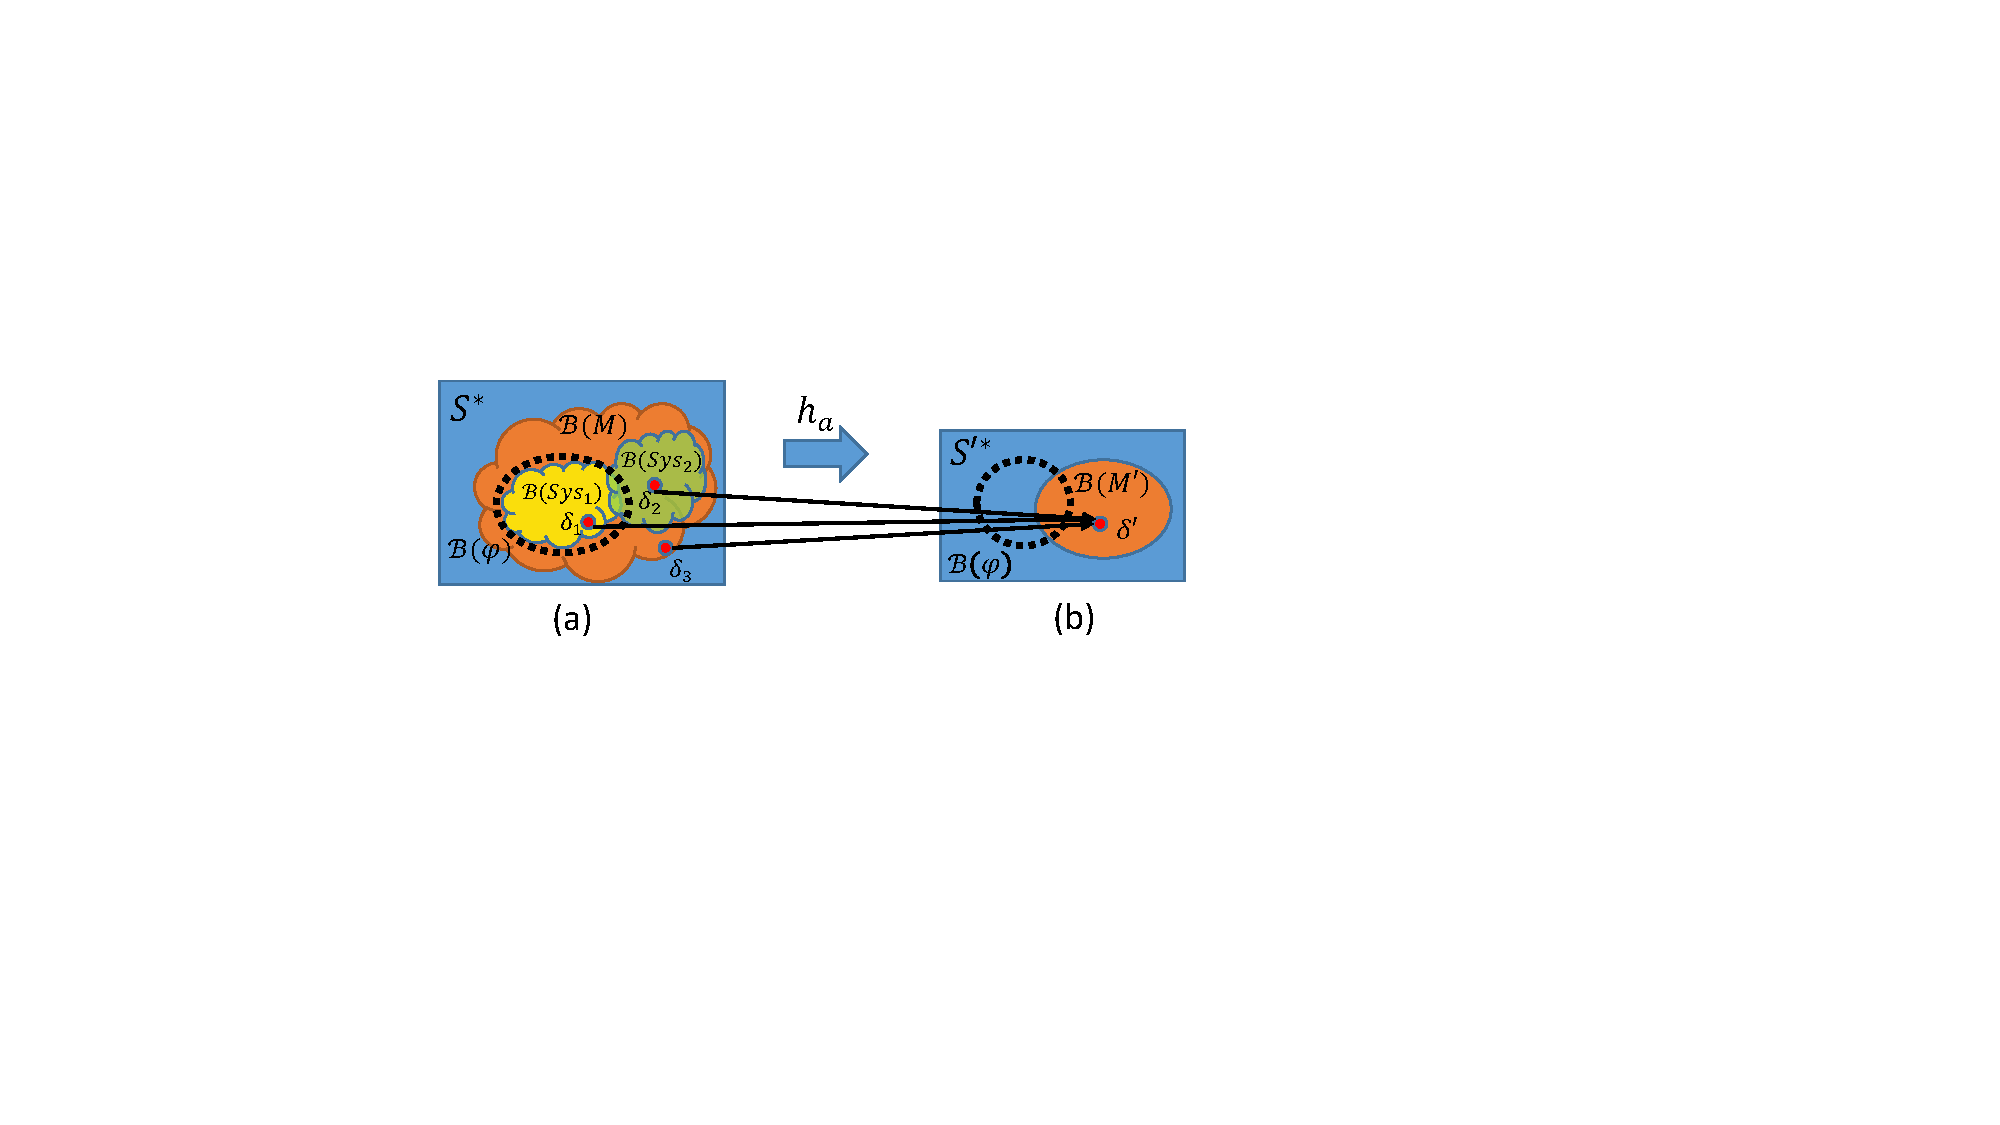
\includegraphics[width=0.7\textwidth]{figs/SysVSEnv.pdf}
		%\vspace{-5pt}
		\caption{\small Two models $Sys1,Sys2$ are over-approximated by model $M$ such that $\{Sys1,Sys2\}\triangleleft_h M$. An over-approximation function $h_a$ is applied to $M$ to obtain $M'$. By model checking the abstract model $M'$ against property $\varphi$ we have $M'\not\models\varphi$ and $\delta'$ is returned as counter-example. However, $\delta'$ corresponds to 3 different behaviors in the original behavior space: $\delta_1$ satisfies $\formula$ and is produced by $Sys1$, $\delta_2$ falsifies $\formula$ and is produced by $Sys2$, and $\delta_3$ falsifies $\varphi$ and belongs to neither behavior space.}
		  %\vspace{-15pt}
		\label{fig:ambiguity}
\end{figure}

\textbf{Validity of a counter-example: }
Behaviors introduced into the over-approximation of a device model are all \emph{spurious}.
For two models such that $M\triangleleft_h M'$, $\delta'$ is spurious if the following condition holds: 
$$\not\exists \delta\in\mathbb{B}(M) \text{ s.t. }\absfun(\delta)=\delta'$$
However, for environment models such that $\{M_1,M_2,...M_n\}\triangleleft_h M'$, and an execution $\delta'\in\mathbb{B}(M')$, the following condition is not enough to prove $\delta'$ is spurious.
$$\forall i\not\exists \delta\in\mathbb{B}(M_i)\text{ s.t. }\absfun(\delta)=\delta'$$
Since there may be a valid environment model $M_c\not\in\{M_1,M_2,...M_n\}$ and $\mathbb{B}(M_c)\subset\mathbb{B}(M')$ and $\delta'\in\mathbb{B}(M_c)$. 
%\hatodoin{no need to repeat the equation, just point to the previous one}
It is thus up to the domain experts to determine the validity of the counter-example.
%\begin{figure}[!b]
%		\centering
%		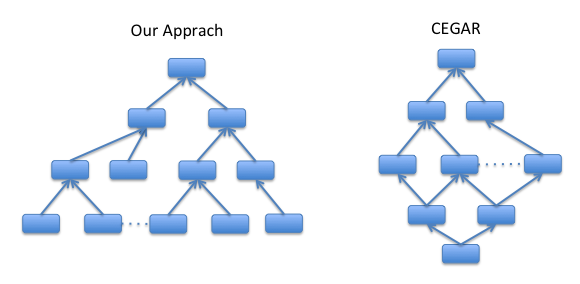
\includegraphics[width=0.6\textwidth]{figs/env_sys.png}
%		%\vspace{-5pt}
%		\caption{\small }
%		  %\vspace{-15pt}
%		\label{fig:distinction}
%\end{figure}
%\subsection{Counter-Example-Guided Abstraction and Refinement (CEGAR)}
%In \cite{CEGAR} the authors proposed a framework to over-approximate the system using proposition abstraction. Upon property violation the abstract counter-example is checked for its validity on the system. If the counter-example is spurious the model is then refined to eliminate the spurious counter-example. This process is then resumed on the refined model until either a valid counter-example returns or no counter-examples are returned.
%
%From the above procedure we can see that CEGAR framework works on system modeling. However, CEGAR cannot be applied for environment modeling for the following reasons. First, the proposition abstraction can not over-approximate multiple models into one abstract model. 
%%Proposition abstraction only abstract the domain of the substates and the dimensions of the state space is unchanged. For environment models with different substates, more aggressive abstraction functions are needed to over-approximate
%With multiple environment models the validity of counter-examples cannot be determined by concretizing them on the set of environment models, as discussed in the last section. If over-approximation is used for environment modeling, there needs to be a more suitable framework to balance the abstraction and refinement of the environment models.
%
%\subsection{Abstraction-tree-based Model Abstraction for Environment Modeling}
%In this paper we propose framework for environment modeling in closed-loop model checking of medical device software. An incomplete set of physiological models are first developed to represent different physiological conditions. 
%
%A set of physiological abstraction rules are then developed based on physiological knowledge, which ensure the physiological relevance of the behaviors introduced into the abstract models. 
%
%Then the rules are applied in certain order onto the set of physiological models, resulting an abstraction tree $G=(V,E)$. Each leaf in the tree is a physiological model and the edges are applications of an abstraction rule. The abstraction tree can then be used as environment models for closed-loop model checking.
%
%The closed-loop requirement $\varphi_c:(\varphi_E\Rightarrow\varphi_P)$ has constraints on the environment in $\varphi_E$. During the abstraction steps, certain sub-states or transitions of the environment models may be removed or merged. If the variables mentioned in $\varphi_E$, which is denoted as $Var(\varphi_E)$, is not a subset of the variables of an environment model $M$, which is denoted as $Var(M)$, the model $M$ is not appropriate for the requirement $\varphi_c$. The first step for closed-loop model checking is to choose the most abstract environment model(s) from the tree which are appropriate for the requirement. These models will be used as the initial environment models $M_E$ during model checking. 
%
%For a system model $M_S$ and a physiological requirement $\varphi_c$, closed-loop model checking is performed such that:
%$$\forall M\in M_E, \text{ check } M||M_S\models\varphi_c$$
%If the requirement is all satisfied, the system model $M_S$ satisfy $\varphi_c$ under environment condition covered by the models in $M_E$. Upon violation of the requirement, the model checker returns a counter-example $\delta_c\in M_c\in M_E$. However, counter-examples at the abstract level are difficult to interpret and there may exists ambiguities. To concretize the counter-example and enumerate possible physiological context, we explore the abstraction tree. Model checking is then performed such that:
%$$\forall M\in Child(M_c), \text{ check } M||M_S\models\varphi_c$$  
%The procedure recurs until 1) the leaves of the tree is reached, or 2) there is no violations in the child nodes. The counter-examples returned from the most refined models are then submitted to the physicians for analysis. 
%In this section we briefly review the notions of abstraction and over-approximation of system.
%Let $M$ be a system model and $S$ be its state space (in Section ??? we give a specific formalism in which our systems are modeled).
%A \emph{trace} $\straj$ of $M$ is an infinite sequence of states produced by $M$: $\straj \in S^\omega$.
%The \emph{behavior} $\beh(M) \subset S^\omega$ of $M$ is then the set of all its possible traces.
%
%Let $AP$ be a set of atomic propositions and $\phi$ be an ACTL$^*$ formula over $AP$ [???].
%ACTL$^*$ is the fragment of CTL$^*$ with only the universal quantifier (``for every path'').
%The set of $M$ traces that satisfy $\phi$ is denoted by $\beh(\phi)$. 
%It holds by definition that if $M$ satisfies $\phi$, then $\beh(M) \subset \beh(\phi)$.
%We write this as $M \models \phi$.
%A model checker takes $M$ and $\phi$ as inputs and either returns SAT, meaning that $M \models \phi$, or returns a \emph{counter-example}, which is a trace $\straj \in \beh(M) \setminus \beh(\phi)$.
%
%An \emph{abstraction function} $\absfun: S \rightarrow S'$ maps the states of $M$ to new \emph{abstract} states.
%We extend it to traces and sets of traces in a natural manner: $\absfun(\straj) =  \absfun(s_0)\absfun(s_1)\ldots$ for $\straj = s_0 s_1\ldots \in S^\omega$,
%and $\absfun(W) = \cup_{\straj \in W}\absfun(\straj)$ for any $W \subset S^\omega$.
%The abstraction function is total (i.e. defined for every $s \in S$) and is such that
%\[R(\beh(M)) \subset \beh(M') \]
%where $\absfun(W) = \cup_{\straj \in W} \absfun(\straj)$.
%Abstraction is used to reduce the size of the state space ($|S'| < |S|$), so that model checking becomes feasible on the new model $M'$ with state space $S'$, while preserving behavior.
%Indeed, if $R(\beh(M)) \subset  \beh(M') $ and $\beh(M') \subset \beh(\phi)$, then it holds that $\beh(M) \subset \beh(\phi)$ and so $M \models \phi$ (here we omit certain technicalities relating to the appropriateness of the abstraction function $\absfun$ to $\phi$. The reader is referred to [Section 3, Clarke JACM] for a good overview).
%
%A \emph{closed loop requirement} is an ACTL$^*$ formula $\formula_C$ of the form $\formula_C :=\formula_E \implies \formula_D$ in which $\formula_E$ describes the open-loop environment behavior that the device encounters, and $\formula_D$ is the closed-loop behavior that the device should achieve. 
%
%A \emph{closed loop requirement} is an ACTL$^*$ formula of the form$\formula_E\Rightarrow \formula_C$ where $\formula_E$ is a specification on the environment model and $\formula_C$ is a specification on the closed-loop model.
%For example, 
%\[\textrm{AtrialSense} \implies \eventually ((\textrm{VentricularSense } ||  \textrm{ VentricularPace }) \land  t \leq 500)\]
% expresses that if the heart displays electrical activity in the atrium (an `atrial sense'), then there should be electrical activity in the ventricles within 500ms (either naturally or as a result of a pacing event).
%
%\subsubsection{Spurious vs physiologically valid counter-examples}
%Suppose a model checker is run on an abstract model $M'$ obtained by abstracting $M$ using some abstraction function $R$.
%If the checking returns a counter example $\straj \in \beh(M')$, two cases are possible:
%either $R^{-1}(x) \in \beh(M)$, or not.
%In the first case, there is no ambiguity: this is a valid counter-example.
%In the second case $R^{-1}(x) \notin \beh(M)$, the trace $\straj$ is usually discarded as being spurious.
%This makes sense if the model $M$ is taken to be the ground truth: i.e. anything not generated by $M$ is not valid behavior. 
%However, when modeling the environment for closed-loop verification, $M$ is only one of many models, none of which is ground truth. 
%That is, it is recognized that there exists physiologically meaningful behavior not captured by any of the models. 
%In this case, we use abstraction functions not only to reduce the size of the state space, but mainly to \emph{introduce, in a systematic manner, physiologically meaningful behavior}. 
%Thus a counter-example $\straj$, while not producable by any of the initial models, may still be a valid example.
%
%\begin{figure}[!t]
%		\centering
%		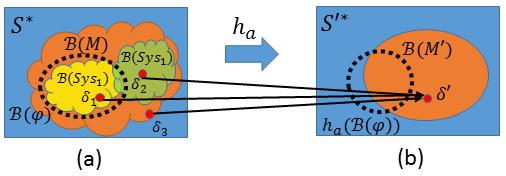
\includegraphics[width=0.8\textwidth]{figs/distinction.png}
%		%\vspace{-5pt}
%		\caption{\small Two models such that $Sys1$ and $Sys2$ are combined into $M$, which is further abstracted into $M'$ using rule $h_a$. By model checking $M'$ against property $\formula$ we have $M'\not\models\formula$ and $\delta$ is returned as counter-example. $\delta$ corresponds to 3 different behaviors in the original behavior space: $\delta_1$ satisfies $\formula$ and is produced by $Sys1$, $\delta_2$ falsifies $\formula$ and is produced by $Sys2$, and $\delta_3$ unsatisfied and invalid}
%		  %\vspace{-15pt}
%		\label{fig:ambiguity}
%\end{figure}
%
